\documentclass[]{../exercices}

\begin{document}
	
	\makeheader{2025}{2026}
	\tdtitle{8}{Réseaux de Neurones}
	
	\begin{exercice}
		On considère un réseau de neurones pour résoudre un problème de régression. Les entrées sont mono-variées $\mathcal{X} \subset \R$ et centrées: $\frac{1}{n} \sum_{i=1}^n x^{(i)} = 0$. L'espace des sorties est $\mathcal{Y} \subset \R$.
		
		Le réseau de neurones étudié est le suivant:
		\begin{itemize}
			\item 1 entrée: $x$
			\item une couche de sortie avec un biais nul (on ne le représentera pas) et un poids $w$.
			\item une fonction d'activation linéaire: $\sigma(z) = z$. On notera $z$ l'entrée de cette fonction d'activation.
			\item 1 sortie: 
		\end{itemize}
		
		On considère la fonction de perte $L: \R \times \R \to \R$ suivante:
		\begin{equation*}
			L(y^{(i)}, \hat{y}^{(i)}) = \left(y^{(i)} - \hat{y}^{(i)}\right)^2
		\end{equation*}
		
		On calculera l'erreur de prédiction $e$ comme suit:
		\begin{equation*}
			e = \frac{1}{n} \sum_{i=1}^n L(y^{(i)}, \hat{y}^{(i)})
		\end{equation*}
		
		
		On dispose des $n$ observations suivantes:
		\begin{table}[h]
			\centering
			\begin{tabular}{|l|c|c|c|c|}
				\hline
				\textbf{Observation} $i$ & 1 & 2 & 3 \\
				\hline
				\textbf{Entrée} $x^{(i)}$ & -1 & 0 & 1 \\
				\hline
				\textbf{Cible}  $y^{(i)}$ & -0.9 & 0.1 & 0.8 \\
				\hline
			\end{tabular}
		\end{table}
		
		On considèrera un algorithme d'optimisation de descente de gradient avec un taux d'apprentissage $\alpha$:
		\begin{equation*}
			w \leftarrow w - \alpha \frac{\partial{e}}{\partial{w}}
		\end{equation*}
		
		\begin{enumerate}
			\item Donner la formulation mathématique du réseau de neurones (passe avant).
			\item Représenter graphiquement l'architecture du réseau de neurones.
			\item Représenter le réseau de neurones sous la forme d'un graphe de calcul en faisant apparaitre l'erreur $e$ et la cible $y$ en plus de la prédiction $\hat{y}$.
			\item On suppose que le poids $w = 0.5$. Calculer la prédiction du réseau neurones avec une passe avant.
			\item Calculer l'erreur $e$ obtenue pour cette passe avant.
			\item Déterminer la dérivée $\displaystyle \frac{\partial{e}}{\partial{\hat{y}}}$. C'est un vecteur colonne de dimension $(n \times 1)$.
			\item Déterminer la dérivée $\displaystyle \frac{\partial{e}}{\partial{\hat{z}}}$. C'est un vecteur colonne de dimension $(n \times 1)$.
			\item Déterminer la dérivée $\displaystyle \frac{\partial{e}}{\partial{w}}$. C'est un scalaire.
			\item Calculer $\displaystyle \frac{\partial{e}}{\partial{w}}$
			\item Recalculer l'erreur $e$ avec les valeurs suivantes de $w$: $0.75$, $0.85$ et $1.0$. Tracer approximativement $e$ en fonction de $w$.
			\item On effectue un pas d'optimisation avec l'algorithme considéré en prenant $\alpha = 0.5$ et $\alpha = 2$ pour un poids initial de $0.5$. Calculer les valeurs de $w$ correspondantes.
			\item Effectuer une nouvelle passe avant avec les deux valeurs de $w$ calculées à la question précédente. Pour chaque passe avant, calculer l'erreur $e$. Que remarquez-vous ?
		\end{enumerate}
	\end{exercice}

\begin{solution}
\begin{enumerate}
    \item La prédiction du réseau de neurones lors de la passe avant peut s'écrire vectoriellement comme :
    \begin{equation*}
        \hat{y} = \sigma(X w)
    \end{equation*}
    Puisque la fonction d'activation est identité/linéaire ($\sigma(z) = z$), on a simplement $\hat{y} = X w$. Pour une observation donnée $i$, on a $\hat{y}^{(i)} = x^{(i)} w$.

    \item Représentation graphique de l'architecture du réseau de neurones :
    \begin{center}
    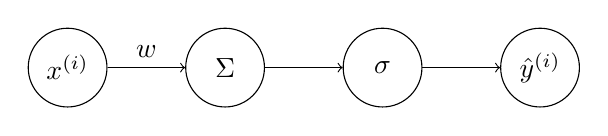
\begin{tikzpicture}[node distance=2cm, scale=1]
        \node[circle, draw, minimum size=1cm] (x) {$x^{(i)}$};
        \node[circle, draw, right of=x, minimum size=1cm] (sum) {$\Sigma$};
        \node[circle, draw, right of=sum, minimum size=1cm] (sigma) {$\sigma$};
        \node[circle, draw, right of=sigma, minimum size=1cm] (y) {$\hat{y}^{(i)}$};
        
        \draw[->] (x) -- node[above] {$w$} (sum);
        \draw[->] (sum) -- (sigma);
        \draw[->] (sigma) -- (y);
    \end{tikzpicture}
    \end{center}

    \item Représentation sous forme de graphe de calcul pour la passe avant et le calcul de l'erreur :
    \begin{center}
    \begin{tikzpicture}[node distance=1.5cm]
        \node (x) {$x$};
        \node[right of=x] (w) {$w$};
        \node[below of=x, xshift=0.75cm] (z) {$z$};
        \node[below of=z] (yhat) {$\hat{y}$};
        \node[below of=yhat] (e) {$e$};
        \node[left of=e] (y) {$y$};
        
        \draw[->] (x) -- (z);
        \draw[->] (w) -- (z);
        \draw[->] (z) -- node[right] {$\sigma$} (yhat);
        \draw[->] (yhat) -- (e);
        \draw[->] (y) -- (e);
    \end{tikzpicture}
    \end{center}

    \item Pour $w = 0.5$, calculons l'entrée de la couche d'activation $Z = X w$ :
    \begin{equation*}
        Z = \begin{pmatrix} -1 \\ 0 \\ 1 \end{pmatrix} (0.5) = \begin{pmatrix} -0.5 \\ 0 \\ 0.5 \end{pmatrix}
    \end{equation*}
    La fonction d'activation étant linéaire, $\hat{Y} = \sigma(Z) = Z$. La prédiction est donc le vecteur $\hat{Y} = (-0.5, 0, 0.5)^T$.

    \item L'erreur quadratique moyenne $e$ s'obtient en moyennant les erreurs individuelles (avec la cible $Y = (-0.9, 0.1, 0.8)^T$) :
    \begin{align*}
        e &= \frac{1}{3} \left[ (-0.9 - (-0.5))^2 + (0.1 - 0)^2 + (0.8 - 0.5)^2 \right] \\
        &= \frac{1}{3} \left[ (-0.4)^2 + (0.1)^2 + (0.3)^2 \right] \\
        &= \frac{1}{3}[0.16 + 0.01 + 0.09] = \frac{0.26}{3} \approx 0.0867
    \end{align*}

    \item La dérivée de l'erreur globale par rapport aux prédictions est un vecteur colonne calculé élément par élément :
    \begin{equation*}
        \left(\frac{\partial e}{\partial \hat{y}}\right)_i = \frac{\partial}{\partial \hat{y}^{(i)}} \left( \frac{1}{n} (y^{(i)} - \hat{y}^{(i)})^2 \right) = \frac{1}{n} \times 2 \times (-1) \times (y^{(i)} - \hat{y}^{(i)}) = \frac{2}{n} (\hat{y}^{(i)} - y^{(i)})
    \end{equation*}
    Vectoriellement, cela s'écrit $\frac{\partial e}{\partial \hat{y}} = \frac{2}{n} (\hat{Y} - Y)$.

    \item En utilisant la règle de dérivation en chaîne, la dérivée de l'erreur par rapport à l'entrée $z$ s'obtient par :
    \begin{equation*}
        \left(\frac{\partial e}{\partial z}\right)_i = \left(\frac{\partial e}{\partial \hat{y}}\right)_i \times \frac{\partial \hat{y}^{(i)}}{\partial z^{(i)}}
    \end{equation*}
    Puisque la fonction d'activation est linéaire ($\sigma(z) = z$), sa dérivée est constante égale à 1 ($\frac{\partial \hat{y}^{(i)}}{\partial z^{(i)}} = 1$). Par conséquent, le vecteur des dérivées par rapport à $z$ est identique :
    $\frac{\partial e}{\partial z} = \frac{\partial e}{\partial \hat{y}}$.

    \item Le poids $w$ intervient dans les prédictions de toutes les observations, la dérivée de l'erreur par rapport à $w$ en est donc la somme :
    \begin{equation*}
        \frac{\partial e}{\partial w} = \sum_{i=1}^n \left(\frac{\partial e}{\partial z}\right)_i \frac{\partial z^{(i)}}{\partial w}
    \end{equation*}
    Comme $z^{(i)} = x^{(i)} w$, on a $\frac{\partial z^{(i)}}{\partial w} = x^{(i)}$. 
    Matriciellement, cela se formule via un produit scalaire : $\frac{\partial e}{\partial w} = X^T \frac{\partial e}{\partial z}$.

    \item Calcul numérique de la dérivée par rapport à $w$ pour $w=0.5$ :
    \begin{align*}
        \frac{\partial e}{\partial w} &= X^T \left( \frac{2}{3} (\hat{Y} - Y) \right) \\
        &= \frac{2}{3} \begin{pmatrix} -1 & 0 & 1 \end{pmatrix} \begin{pmatrix} -0.5 - (-0.9) \\ 0 - 0.1 \\ 0.5 - 0.8 \end{pmatrix} \\
        &= \frac{2}{3} \begin{pmatrix} -1 & 0 & 1 \end{pmatrix} \begin{pmatrix} 0.4 \\ -0.1 \\ -0.3 \end{pmatrix} \\
        &= \frac{2}{3} (-1 \times 0.4 + 0 \times (-0.1) + 1 \times (-0.3)) = \frac{2}{3} (-0.7) \approx -0.467
    \end{align*}

    \item Recalcul de l'erreur globale pour d'autres valeurs de $w$ :
    \begin{itemize}
        \item $w = 0.75 \implies \hat{Y} = (-0.75, 0, 0.75)^T$. \\
        $e = \frac{1}{3} \left[ (-0.9 - (-0.75))^2 + 0.1^2 + (0.8 - 0.75)^2 \right] = \frac{1}{3}((-0.15)^2 + 0.1^2 + 0.05^2) = 0.0116$
        \item $w = 0.85 \implies \hat{Y} = (-0.85, 0, 0.85)^T$. \\
        $e = \frac{1}{3} \left[ (-0.9 - (-0.85))^2 + 0.1^2 + (0.8 - 0.85)^2 \right] = \frac{1}{3}((-0.05)^2 + 0.1^2 + (-0.05)^2) = 0.005$
        \item $w = 1.0 \implies \hat{Y} = (-1, 0, 1)^T$. \\
        $e = \frac{1}{3} \left[ (-0.9 - (-1))^2 + 0.1^2 + (0.8 - 1)^2 \right] = \frac{1}{3}(0.1^2 + 0.1^2 + (-0.2)^2) = 0.02$
    \end{itemize}
    On observe que la fonction de perte forme une parabole (strictement convexe) avec un minimum situé autour de $w = 0.85$ :
    \begin{center}
    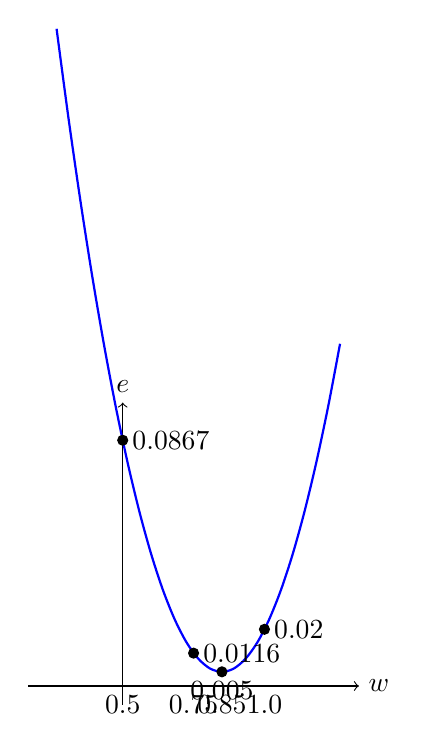
\begin{tikzpicture}[scale=1.2]
        \draw[->] (0.5,0) -- (4,0) node[right] {$w$};
        \draw[->] (1.5,-0.2) -- (1.5,3) node[above] {$e$};
        
        \draw[domain=0.8:3.8, smooth, variable=\w, blue, thick] plot ({\w}, {30*(2/3*((\w/3)-0.85)^2 + 0.005)});
        
        \filldraw (0.5*3, {30*0.0867}) circle (1.5pt) node[right] {$0.0867$};
        \filldraw (0.75*3, {30*0.0116}) circle (1.5pt) node[right] {$0.0116$};
        \filldraw (0.85*3, {30*0.005}) circle (1.5pt) node[below] {$0.005$};
        \filldraw (1.0*3, {30*0.02}) circle (1.5pt) node[right] {$0.02$};
        
        \node[below] at (0.5*3,0) {$0.5$};
        \node[below] at (0.75*3,0) {$0.75$};
        \node[below] at (0.85*3,0) {$0.85$};
        \node[below] at (1.0*3,0) {$1.0$};
    \end{tikzpicture}
    \end{center}

    \item Mise à jour des poids avec l'algorithme de descente de gradient depuis $w=0.5$ :
    \begin{itemize}
        \item Pour $\alpha = 0.5$ : $w \leftarrow 0.5 - 0.5 \times (-0.467) = 0.5 + 0.2335 = 0.7335$
        \item Pour $\alpha = 2$ : $w \leftarrow 0.5 - 2 \times (-0.467) = 0.5 + 0.934 = 1.434$
    \end{itemize}

    \item Évaluation de l'erreur après la mise à jour :
    \begin{itemize}
        \item Pour $w = 0.7335$ : $\hat{Y} = (-0.7335, 0, 0.7335)^T$. \\
        $e \approx \frac{1}{3} ((-0.1665)^2 + 0.1^2 + (0.0665)^2) \approx 0.014$ \\
        L'erreur diminue de $0.0867$ à $0.014$. Le gradient a permis de converger vers le minimum.
        \item Pour $w = 1.434$ : $\hat{Y} = (-1.434, 0, 1.434)^T$. \\
        $e \approx \frac{1}{3} (0.534^2 + 0.1^2 + (-0.634)^2) \approx 0.232$ \\
        L'erreur augmente brutalement de $0.0867$ à $0.232$. Avec $\alpha=2$, le taux d'apprentissage est trop grand, \textbf{l'algorithme diverge}.
    \end{itemize}
\end{enumerate}
\end{solution}

	\begin{exercice}
		Dans cet exercice on étudiera les fonctions d'activation suivantes pour $z \in R$:
		\begin{equation*}
			\begin{aligned}
				\sigma(z) &= \frac{1}{1 + e^{(-z)}} \\
				\tanh(z) &= \frac{1 - e^{-2 z}}{1 + e^{- 2 z}} \\
				\operatorname{ReLU}(z) &= \max{(z, 0)}
			\end{aligned}
		\end{equation*}
		
		\begin{enumerate}
			\item Démontrer que $\sigma'(z) = \sigma(z) \left(1 - \sigma(z)\right)$.
			\item Démontrer que $\tanh'(z) = 1 - \tanh^2(z)$.
			\item Calculer la dérivée de $\operatorname{ReLU}(z)$. On supposera que la dérivée est nulle en $z = 0$.
			\item Pour les trois fonctions, calculer les dérivées en $z=-5$, $z=0$ et $z=5$.
			\item Si un réseau dispose de 10 couches, que se passe-t-il lors de la passe arrière si jamais les fonctions d'activations sont toujours sollicitées dans une zone $z=5$ ?
			\item Pour un réseau de neurones simple à une couche cachée avec une fonction ReLU, que se passe-t-il si lors de la passe avant toutes les entrées de ReLU sont négatives.
			\item Discuter des potentiels problèmes que les réponses aux question 5 et 6 pourraient causer sur l'apprentissage.
		\end{enumerate}
		
	\end{exercice}

\begin{solution}
\begin{enumerate}
    \item La dérivée de la fonction sigmoïde $\sigma(z) = \frac{1}{1 + e^{-z}} = (1 + e^{-z})^{-1}$ s'obtient comme suit :
    \begin{align*}
        \sigma'(z) &= -1 \times (-e^{-z}) \times (1 + e^{-z})^{-2} \\
        &= \frac{e^{-z}}{(1 + e^{-z})^2} \\
        &= \frac{1}{1 + e^{-z}} \times \frac{e^{-z}}{1 + e^{-z}} \\
        &= \sigma(z) \times \frac{1 + e^{-z} - 1}{1 + e^{-z}} \\
        &= \sigma(z) \left( \frac{1 + e^{-z}}{1 + e^{-z}} - \frac{1}{1 + e^{-z}} \right) \\
        &= \sigma(z) (1 - \sigma(z))
    \end{align*}

    \item La dérivée de la tangente hyperbolique $\tanh(z) = \frac{1 - e^{-2z}}{1 + e^{-2z}}$ s'obtient avec la formule de dérivation d'un quotient $\left(\frac{u}{v}\right)' = \frac{u'v - uv'}{v^2}$ :
    \begin{align*}
        \tanh'(z) &= \frac{2e^{-2z}(1 + e^{-2z}) - (1 - e^{-2z})(-2e^{-2z})}{(1 + e^{-2z})^2} \\
        &= \frac{2e^{-2z} + 2e^{-4z} + 2e^{-2z} - 2e^{-4z}}{(1 + e^{-2z})^2} = \frac{4e^{-2z}}{(1 + e^{-2z})^2}
    \end{align*}
    En parallèle, évaluons l'expression $1 - \tanh^2(z)$ :
    \begin{align*}
        1 - \tanh^2(z) &= 1 - \frac{(1 - e^{-2z})^2}{(1 + e^{-2z})^2} \\
        &= \frac{(1 + e^{-2z})^2 - (1 - e^{-2z})^2}{(1 + e^{-2z})^2} \\
        &= \frac{(1 + 2e^{-2z} + e^{-4z}) - (1 - 2e^{-2z} + e^{-4z})}{(1 + e^{-2z})^2} \\
        &= \frac{4e^{-2z}}{(1 + e^{-2z})^2}
    \end{align*}
    On a donc bien démontré que $\tanh'(z) = 1 - \tanh^2(z)$.

    \item La fonction d'activation ReLU est définie par $\operatorname{ReLU}(z) = \max(z, 0)$. Sa dérivée vaut :
    \begin{equation*}
        \operatorname{ReLU}'(z) = \begin{cases}
            1 & \text{si } z > 0 \\
            0 & \text{si } z \leq 0 \quad (\text{selon l'hypothèse de l'énoncé en } z=0)
        \end{cases}
    \end{equation*}

    \item Tableau comparatif des dérivées pour les différentes valeurs de $z$ :
    \begin{table}[h]
        \centering
        \begin{tabular}{|c|c|c|c|}
            \hline
            $z$ & $\sigma'(z)$ & $\tanh'(z)$ & $\operatorname{ReLU}'(z)$ \\
            \hline
            -5 & $\approx 0.0067$ & $\approx 0.0002$ & 0 \\
            \hline
            0 & $0.25$ & 1 & 0 \\
            \hline
            5 & $\approx 0.0067$ & $\approx 0.0002$ & 1 \\
            \hline
        \end{tabular}
    \end{table}

    \item Lors de la passe arrière (backpropagation), les gradients sont rétro-propagés en multipliant les dérivées locales des couches. Si les activations d'un réseau profond de 10 couches tombent systématiquement dans la zone $z=5$, les gradients pour ReLU sont de 1, et donc se propagent de manière intacte. \textbf{Par contre}, pour les fonctions $\sigma$ et $\tanh$, leurs dérivées valent une fraction infime (ex: $0.0067$ ou $0.0002$). Le produit de ces petites valeurs à chaque couche provoque une \textbf{disparition du gradient} (vanishing gradient) qui tend presque vers $0$ sur les premières couches.

    \item Pour un neurone dont l'activation est ReLU, si ses entrées sont toutes négatives lors de la passe avant, la dérivée $\operatorname{ReLU}'$ vaudra 0 pour toutes ses données. Ainsi, la rétropropagation donnera un gradient nul par rapport à ce neurone : ses poids ne seront jamais mis à jour. Le neurone ne pourra plus rien apprendre, on parle alors de \textbf{neurone mort} (dead ReLU).

    \item Conséquences pour l'apprentissage : Les réseaux de neurones \textbf{n'apprennent plus} et leur mise à jour stagne lorsque les gradients disparaissent (que ce soit à cause de l'écrasement des gradients des sigmoïdes aux bornes, ou par annulation stricte à cause des neurones ReLU morts). C'est pourquoi le choix des fonctions d'activation et l'initialisation des poids sont critiques.
\end{enumerate}
\end{solution}

	\begin{exercice}
		On considère la couche de sortie d'un réseau de neurones pour un problème de classification binaire. Le réseau prédit une probabilité $\hat{y} \in ]0, 1[$ en utilisant une fonction d'activation de type logistique sur cette couche de sortie. On notera $z$ l'entrée de la fonction logistique: $\sigma(z) = \hat{y}$. Les classes vraies sont notées $y \in \{0, 1\}$. Le réseau est entraîné en utilisant une fonction de perte d'entropie croisée binaire pour une observation $i$:
		\begin{equation*}
			L(y^{(i)}, \hat{y}^{(i)}) = - \left[ y^{(i)} \ln(\hat{y}^{(i)}) + (1 - y^{(i)}) \ln(1 - \hat{y}^{(i)}) \right]
		\end{equation*}
		L'erreur de prédiction $e$ est calculée comme suit pour les $n$ observations des données d'apprentissage:
		\begin{equation*}
			e = \frac{1}{n} \sum_{i=1}^n L(y^{(i)}, \hat{y}^{(i)})
		\end{equation*}
		\begin{enumerate}
			\item Calculer la dérivée $\frac{\partial{L(y^{(i)}, \hat{y}^{(i)})}}{\partial{\hat{y}^{(i)}}}$
			\item En déduire la dérivée $\frac{\partial{e}}{\partial{\hat{y}}}$
			\item Démontrer que $\frac{\partial{e}}{\partial{z}} = \frac{1}{n}\left(\hat{y} - y\right)$
			\item Déduire de ce résultat une simplification possible de l'algorithme d'apprentissage d'un réseau de neurones pour un problème de classification binaire.
		\end{enumerate}
	\end{exercice}

\begin{solution}
\begin{enumerate}
    \item La dérivée de la fonction de perte d'entropie croisée pour une observation $i$ par rapport à la prédiction $\hat{y}^{(i)}$ :
    \begin{align*}
        \frac{\partial L(y^{(i)}, \hat{y}^{(i)})}{\partial \hat{y}^{(i)}} &= - \left[ y^{(i)} \frac{\partial \ln(\hat{y}^{(i)})}{\partial \hat{y}^{(i)}} + (1 - y^{(i)}) \frac{\partial \ln(1 - \hat{y}^{(i)})}{\partial \hat{y}^{(i)}} \right] \\
        &= - \left[ y^{(i)} \frac{1}{\hat{y}^{(i)}} + (1 - y^{(i)}) \frac{-1}{1 - \hat{y}^{(i)}} \right] \\
        &= - \frac{y^{(i)}}{\hat{y}^{(i)}} + \frac{1 - y^{(i)}}{1 - \hat{y}^{(i)}}
    \end{align*}

    \item L'erreur de prédiction $e$ étant la moyenne des pertes, sa dérivée par rapport au vecteur des prédictions $\hat{y}$ est le vecteur colonne contenant la dérivée locale divisée par le nombre d'échantillons $n$ :
    \begin{equation*}
        \frac{\partial e}{\partial \hat{y}} = \frac{1}{n} \left( -\frac{y}{\hat{y}} + \frac{1 - y}{1 - \hat{y}} \right)
    \end{equation*}

    \item La dérivée de l'erreur par rapport à l'entrée non-activée (logit) $z$ s'obtient par la règle de dérivation en chaîne (chain rule). Pour une observation :
    \begin{equation*}
        \frac{\partial e}{\partial z^{(i)}} = \frac{\partial e}{\partial \hat{y}^{(i)}} \times \frac{\partial \hat{y}^{(i)}}{\partial z^{(i)}}
    \end{equation*}
    Puisque $\hat{y}^{(i)} = \sigma(z^{(i)})$ (la fonction logistique), on a démontré que $\frac{\partial \hat{y}^{(i)}}{\partial z^{(i)}} = \hat{y}^{(i)} (1 - \hat{y}^{(i)})$. En remplaçant et en développant :
    \begin{align*}
        \frac{\partial e}{\partial z^{(i)}} &= \frac{1}{n} \left( - \frac{y^{(i)}}{\hat{y}^{(i)}} + \frac{1 - y^{(i)}}{1 - \hat{y}^{(i)}} \right) \times \hat{y}^{(i)} (1 - \hat{y}^{(i)}) \\
        &= \frac{1}{n} \left[ - y^{(i)} \frac{\hat{y}^{(i)} (1 - \hat{y}^{(i)})}{\hat{y}^{(i)}} + (1 - y^{(i)}) \frac{\hat{y}^{(i)} (1 - \hat{y}^{(i)})}{1 - \hat{y}^{(i)}} \right] \\
        &= \frac{1}{n} \left[ -y^{(i)} (1 - \hat{y}^{(i)}) + (1 - y^{(i)}) \hat{y}^{(i)} \right] \\
        &= \frac{1}{n} \left[ -y^{(i)} + y^{(i)} \hat{y}^{(i)} + \hat{y}^{(i)} - y^{(i)} \hat{y}^{(i)} \right] \\
        &= \frac{1}{n} \left( \hat{y}^{(i)} - y^{(i)} \right)
    \end{align*}
    La formulation vectorisée pour l'ensemble des données est alors :
    \begin{equation*}
        \frac{\partial e}{\partial z} = \frac{1}{n}(\hat{y} - y)
    \end{equation*}

    \item La forme mathématique finale de la dérivée de l'erreur par rapport au logit $z$ est remarquablement simple et linéaire vis-à-vis de l'erreur de prédiction, et surtout, ne fait apparaître \textbf{aucun terme exponentiel ni quotient}. 
    
    Il est donc beaucoup plus facile et numériquement plus stable d'inclure le calcul de la sigmoïde directement au sein de la fonction de perte. C'est pour cette raison que les librairies de Deep Learning pour la classification binaire omettent l'activation sigmoïde dans la passe avant des réseaux et utilisent une entropie croisée directement sur les logits (\textit{BCEWithLogitsLoss}) comme fonction de perte. Pour l'inférence (utilisation du modèle), il suffit de réappliquer manuellement une sigmoïde sur les sorties pour extraire les probabilités finales.
\end{enumerate}
\end{solution}

\end{document}
